\documentclass[a4paper,conference]{IEEEtran}

% Packages
\usepackage[pdftex]{graphicx}				% Graphics
\DeclareGraphicsExtensions{.pdf,.jpeg,.jpg,.png}
\usepackage{tabularx}						% Tables
\usepackage{amsmath}						% Math
\usepackage{mathtools}						% Extra Mathematische Symbole
\usepackage{algorithmic}					% Algorithmics
\usepackage{cleveref}						% Citations
\usepackage{bytefield}						% Bytefield
\usepackage{tikz}							% tikz-figures
\usetikzlibrary{positioning,arrows,automata}

\begin{filecontents}{tcp.data}
#Transmission round		Congestion Window Size
1		1
2		2
3		4
4		8
5		16
6		32
7		16
8		17
9		18
10		19
11		20
12		10
13		5
14		6
15		7
\end{filecontents}


% correct bad hyphenation here
\hyphenation{op-tical net-works semi-conduc-tor}

\bibliographystyle{IEEEtran}

\begin{document}

% paper title
\title{The Origins of Congestion and\\Network Assisted End-to-End Congestion Control}


% author
\author{\IEEEauthorblockN{Til Mohr}
\IEEEauthorblockA{RWTH Aachen University\\til.mohr@rwth-aachen.de}}

% use for special paper notices
%\IEEEspecialpapernotice{(Invited Paper)}

% make the title area
\maketitle
\IEEEpeerreviewmaketitle

\begin{abstract}
This article presents the most common origins of network congestion, how different types of algorithms perceive and handle congestion and what obstacles they face.
\end{abstract}

\section{Introduction}
Congestion was, is and always will be a problem on the Internet, appearing in various forms with different symptoms causing minor, but also major challenges. Data sent over the internet is split up in smaller packets that all try to reach their destination the fastest, whether it is by going the shortest or the least congested route. In an optimal network all computers, servers etc. would have a direct link to each other, thus reducing the importance of bandwidth and  consequently removing the need for buffers at all. However, the larger the network would get, the amount of connections would grow quadratic.
\\Networks today consist of network nodes (routers, switches, ...) which all try to route internet packets as quick as possible whilst keeping the required hardware to a minimum. Ideally there would be a steady flow of packets being transmitted at maximum rate. However, when a internet node receives a packet while the outgoing connection still is in use, the packet has to be stored in a buffer until the outgoing connection freed up again. Therefore, those storage units are essential to every node on a network, but without proper management even well-sized buffers could lead to network problems like packet-loss, jitter and connection delay \cite{appenzeller2004sizing}	.
\\This paper will present origins of network congestion and analyze how different types of algorithms try to avoid and minimize congestion.

\section{Origins of Congestion}
With the ever-growing amount of internet services not only data-centers, but the whole internet in general face new problems with each packet sent. Therefore, the global reduction of those complications are an important task to improve the quality of all internet services. However, as it is for solving any problem, the origin of those problems must be identified first.
\\Network delay can generally speaking be categorized into three different types of delay \cite{gettys2012bufferbloat}:

\begin{itemize}
\item 
\textit{Transmission delay} describes the delay of transmitting data packets between two internet nodes. Typically, packets sent from a origin to a destination node are sent over various different internet nodes, all of which could have a different bandwidth. Therefore, a packet send from \textbf{node 1} to \textbf{node n} over \textbf{nodes 2 to n-1} cannot be sent at a faster rate than the lowest bandwidth on the packets path (bottleneck) [Figure \ref{fig:transmission delay}].\[Rate_{max} = \min\{bandwidth_{i}\mid i\in\{1,...,n-1\}\}\]

\item
\textit{Processing delay} is the time needed to process an individual packet by an internet node. This usually means processing the packets IP header, finding its destination and possibly queuing it in buffers.

\item
\textit{Queuing delay} is the time a package spent waiting for it to be processed or transmitted.
\end{itemize}
\begin{figure}
	\begin{center}
	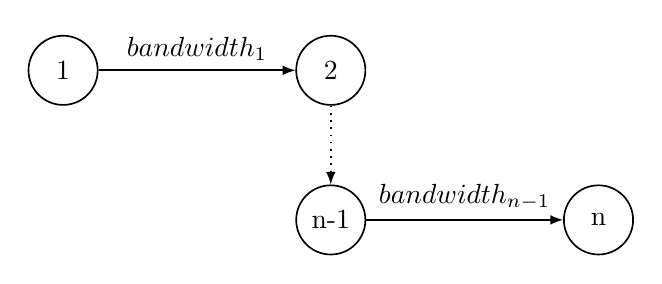
\begin{tikzpicture}[->, >=latex, node distance = 1cm and 2.5cm, semithick]
		% Nodes
		\node[state] (A)  			   	{1};
		\node[state] (B) [right=of A] 	{2};
		\node[state] (C) [below=of B] 	{n-1};
		\node[state] (D) [right=of C] 	{n};
		%Arrows
		\path	
		(A) edge [above] node {$bandwidth_{1}$} (B)
		(B) edge [dotted] (C)
		(C) edge [above] node {$bandwidth_{n-1}$} (D)
		;
	\end{tikzpicture}
	\end{center}
	\caption{Path a packet takes through the network}
	\label{fig:transmission delay}
\end{figure}

Whereas processing delay is almost not noticeable and transmission delay could be improved by upgrading cables or transmission protocols, queuing delay has various causes and therefore is the  most difficult one to reduce. There are many different ways to implement buffers in a network node and the effectiveness of each implementation varies from where it is used. Traffic in residential network nodes for example differ from nodes used in large data-centers in every aspect, thus hardware and software in those components should be adjusted accordingly.
\\Sizing buffers is a complex task. On the one hand read and write times should as short as possible to minimize additional delay. On the other hand buffers should be as big as needed to be robust for future network changes and therefore store lots of data if needed while also keeping in mind the requirements congestion detection algorithms have in order to adjust for congestion accordingly \cite{staff2012bufferbloat}. Unifying those goals is very challenging as it leads to increasing costs and physical space occupied by those buffers. Additionally, a 2004 paper by Appenzeller found that 99\% of buffers in network nodes, which were sized on a rule-of-thumb rule based on the TCP protocol \cite{villamizar1994high}, could be removed without losing, but rather gaining performance \cite{appenzeller2004sizing}. Clearly, balancing speed and size is difficult and thus buffer sizes should be adjusted to their area of use accordingly.
\begin{figure}
  \centering
    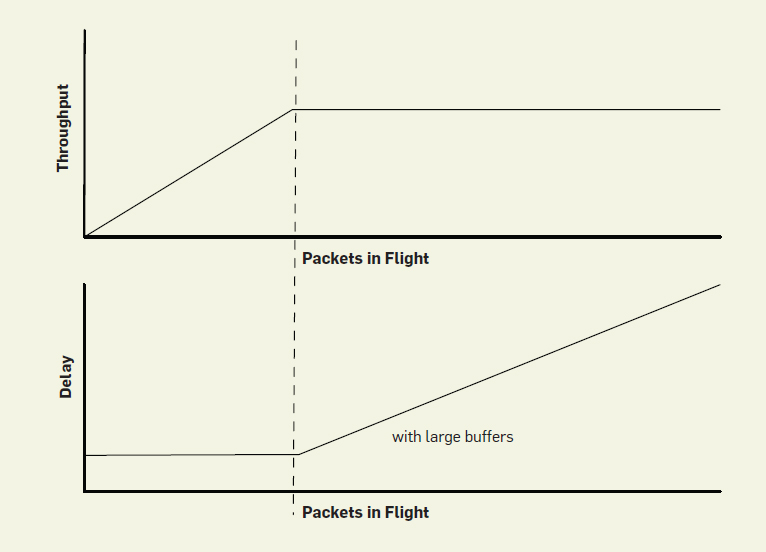
\includegraphics[width=0.9\linewidth]{figures/Throughput-Delay}
  \caption{Relationship between throughput and delay \cite{gettys2012bufferbloat}}
  \label{fig:throughput-delay-relationship}
\end{figure}
\\This isn't the only major cause of queuing delay. Without proper buffer management even nodes with well sized buffers will experience performance loss. Proper queue management is able to compensate for the unpredictable fluidity of network traffic. It is an difficult task to buffer the right amount of packages to keep transmission flow consistent over time.
As the number of packets being transmitted grows, the \textit{throughput} of the network node increases until packets are being transmitted at bottleneck rate. After this, the transmission rate cannot increase anymore, which leads to packets being buffered along their path to prevent them being lost [Figure \ref{fig:throughput-delay-relationship}]\cite{gettys2012bufferbloat}. If the incoming amount of traffic keeps to exceed the amount of outgoing traffic, those buffers will fill up (\textit{over-buffering}), which will eventually lead to \textit{bufferbloat} \cite{Allman13commentson,6886125}.

\subsection*{Bufferbloat}
Bufferbloat refers to frequently full and excessively large buffers in internet nodes. This leads to partly unnecessary network delay and damages congestion avoidance algorithms, such as classic TCP \cite{gettys2012bufferbloat,chen2014bufferbloat}. Buffering is needed to provide space to queued packets waiting for transmission resulting in a minimization of packet loss. In the past however, buffer sizes were smaller than today's thus less packets could be queued and more were dropped, signaling transmission protocols the presence of congestion in this node, so those protocols can adjust. With memory getting cheaper over the years, buffers saw an increase in size. This has the negative impact, that more packets can be queued before any are dropped, thus those adjustments of congestion avoidance protocols kick in later than usual. Thus, buffers are being filled in the whole network which results in an extreme increase in network delay (\textit{latency}) and fluctuation (\textit{jitter}) \cite{gettys2012bufferbloat,staff2012bufferbloat,chen2014bufferbloat}.
\\So Services, which require low latency at a high data-rate, such as Streaming, will experience a decrease in quality.


\section{Congestion Avoidance}
As already mentioned, congestion detection algorithms make up an important part in congestion avoidance protocols. \textit{TCP} is such an protocol, based on the transport layer, which adapts its send rate according to available network bandwidth \cite{1209197,jacobson1992tcp}. To fully understand, how TCP's congestion avoidance algorithm functions, you will have to understand how TCP works. TCP lives on the transport layer. It communicates with the application layer via ports, splits up data into packets (and vice versa), and transmits those packages over the network with the use of the internet protocol, thus TCP is often also referred to as \textit{TCP/IP}. It is the interface between network components. Each of those communication packages have different purposes, but underlay the same structure - the protocol header. The TCP header is split up into multiple segments [Figure \ref{fig:TCP_Header}]\cite{jacobson1992tcp,huston2000tcp}:
\begin{figure}
\centering
\begin{bytefield}[bitheight=2.2\baselineskip]{32}
	\bitbox{16}{Source Port} & \bitbox{16}{Destination Port} \\
	\bitbox{32}{Sequence Number} \\
	\bitbox{32}{Acknowledgment Number} \\
	\bitbox{4}{Data Offset} & \bitbox{6}{Reserved} &
\bitbox{1}{\tiny U\\R\\G} & \bitbox{1}{\tiny A\\C\\K} &
\bitbox{1}{\tiny P\\S\\H} & \bitbox{1}{\tiny R\\S\\T} &
\bitbox{1}{\tiny S\\Y\\N} & \bitbox{1}{\tiny F\\I\\N} &
\bitbox{16}{Window Size} \\
\bitbox{16}{Checksum} & \bitbox{16}{Urgent Pointer} \\
\bitbox{32}{Options} \\
\bitbox{32}{Data}
\end{bytefield}
\caption{TCP Header}
\label{fig:TCP_Header}
\end{figure}
\begin{itemize}
\item \textit{Source Port} and \textit{Destination Port} specify the ports on which TCP should communicate with the application layer.

\item The \textit{Sequence Numbers} and \textit{Acknowledgment Numbers} specify how much data has been sent so far. All bytes in a TCP connection are numbered in increasing order, with both sides of the connection keeping track of those numbers. This way packet loss can be detected.

\item TCP can set six different bit-flags in its header. The most important one is the \textit{ACK} flag (Acknowledgement bit). It is used whenever a packet receives the destination and an acknowledgement packet has to be sent back. The \textit{SYN} and \textit{FIN} flags initialize and terminate a connection.

\item The \textit{Window Size} is the maximum amount of data (in bytes) a receiver is willing to receive at any time. It is being negotiated at the initialization of a new connection and can only be negotiated again with the \textit{SYN} flag set. It is important to set it appropriately to prevent unnecessary packet loss or delay, as the receiver couldn't process the data in time \cite{jacobson1992tcp}.
\end{itemize}
TCP uses a handshake system. Whenever a client sends a data packet to the server, the server waits until it has received enough data (specified by the window size), and then sends back an acknowledgment package, signaling the successful transmission of data. There are also other handshake operations used, for example for establishing or terminating a connection, however those have no further importance to the congestion avoidance protocol \cite{1209197,jacobson1992tcp,huston2000tcp,jacobson1995congestion}.

\subsection{Perceiving Congestion}
Both partners of a connection are either a sender or a receiver. The sender keeps track of the time it takes from when a package sent until the acknowledgment is received. This is also known as \textit{round-trip time} (RTT), where a large RTT can indicate some congestion along the path. Some variances of TCP make use of this feature in their congestion avoidance algorithms, yet classic TCP does not \cite{huston2000tcp,jacobson1995congestion}. RTT also plays an very important role in the detection of packet loss, which further imply congestion. The sender side keeps track of the RTT while it is being measured and compares it to the \textit{retransmission timeout} (RTO) \cite{jacobson1992tcp}. RTO time is being calculated by estimating the mean and variance of the RTT. Whenever 	packets are not acknowledged within this RTO intervall, the package is being detected as lost and will be retransmitted. Therefore, it is essential to TCP performance, that the RTO is being determined accurately, as a too low RTO could prompt unnecessary retransmissions and too high RTO could slow down the application TCP is serving \cite{huston2000tcp,jacobson1995congestion}.\\
Note however, a high RTT can also have other causes than packet loss or congestion. A short term drastic decrease in the receivers processing performance can lead to packets being buffered at the receivers end for a prolonged period of time, thus resulting in a higher RTT \cite{huston2000tcp}.

\subsection{Adjusting for Congestion}
To prevent congestion altogether, packet flow inside a network would have to be conservative, i.e. a new packet isn't being sent into the network before an old packet leaves the network. A connection in this state is also being described as being \textit{in equilibrium} \cite{jacobson1992tcp}. Whenever a connection is in equilibrium, congestion in the network cannot be caused by this TCP connection, thus also controlling congestion. TCPs congestion avoidance algorithm can be categorized into three sub-algorithms, that all have the goal to keep the connection in equilibrium, no matter how congestion was perceived. Here, a variable called \textit{congestion window} (cwnd) has an important role. It describes the maximum amount of packages send during a interval. An additional mechanism of keeping a connection in equilibrium is, that each acknowledgement package received by the sender opens the space for a new package to be sent into the network \cite{jacobson1992tcp}.

\subsubsection*{Slow-Start}
The \textit{slow-start} algorithm is used when a connection has just been established or when multiple packet losses were detected. The cwnd variable is set to one package per estimated RTT, because no information about network congestion has been collected yet. Whenever an acknowledgment package is being received, cwnd will increase by one package. This exponential growth in packages helps to get the packet send rate to the maximum the network can handle quite quickly, resulting in almost immediately maximum network performance \cite{jacobson1992tcp}. Slow-start will only increase if cwnd

\subsubsection*{Adaption}
When the network is congested, buffers in network nodes will fill up exponentially \cite{jacobson1992tcp}. Therefore, the network can only stabilize if the amount of packets sent decreases at least as quickly as the queues are growing. The formula \cite{jacobson1992tcp} \[cwnd_{i+1}=d*cwnd_{i}, 0<d<1\] has an exponential decrease over time, thus resulting in the network recovering.\\
If the network isn't congested, the sender should try to raise cwnd slowly to reach the networks maximum throughput again. A multiplicative, exponential increase over time, like the slow-start algorithm isn't the best choice here. Increasing the amounts of packets sent drastically while cwnd still is high can result in the network being challenge the networks capacity, resulting in heavy congestion. Therefore, the best option to raise cwnd to its limits is an additive increase \cite{jacobson1992tcp}:\[cwnd_{i+1}=cwnd_{i} + u\] Van Jacobson proposes in his 1992 paper about TCP congestion avoidance that $d$ will be set to $\frac{1}{2}$ and $u$ will be set to $\frac{1}{cwnd_{i}}$. Thus, cwnd can only increase by a maximum of one packet per RTT leading to a smooth approach to the networks limit \cite{jacobson1992tcp}.

\begin{figure}
  \centering
    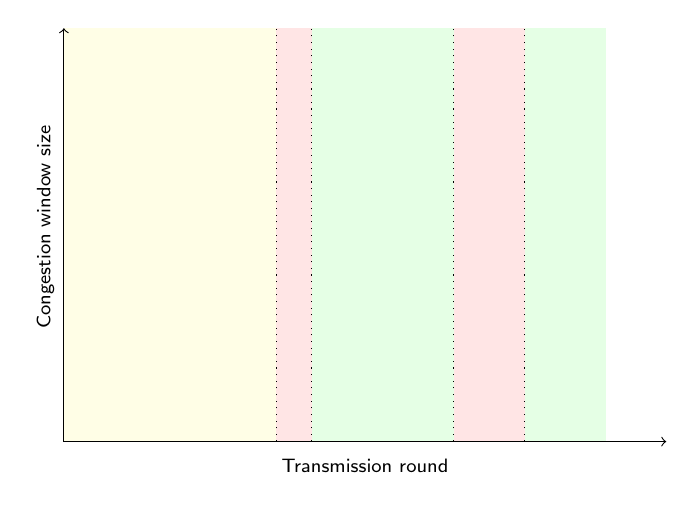
\begin{tikzpicture}[y=.15cm, x=.45cm,font=\sffamily]
    	% Ranges and dotted lines
    	\fill[yellow!10]	(0,0) rectangle (6,35);
    	\fill[red!10] 		(6,0) rectangle (7,35);
    	\fill[green!10] 	(7,0) rectangle (11,35);
    	\fill[red!10]		(11,0) rectangle (13,35);
    	\fill[green!10]		(13,0) rectangle (15.3,35);
    	\draw[dotted] 		(6,0) -- (6,35);
    	\draw[dotted] 		(7,0) -- (7,35);
    	\draw[dotted] 		(11,0) -- (11,35);
    	\draw[dotted] 		(13,0) -- (13,35);
    	% Axis
    	\draw[->] 			(0,0) -- coordinate (x axis mid) (17,0);
    	\draw[->] 			(0,0) -- coordinate (y axis mid) (0,35);
    	% Labels
    	\node[below=0.1cm] at (x axis mid) {\scriptsize Transmission round};
    	\node[rotate=90, above=0.1cm] at (y axis mid) {\scriptsize Congestion window size};
    	% Plot
    	\draw plot[mark=*]
    		file {tcp.data};
    \end{tikzpicture}
  \caption{TCP congestion avoidance protocols. Yellow represents the slow-start sequence, red and green symbolize detected congestion}
  \label{fig:tcp_congestion_avoidance_protocols}
\end{figure}



\section{Network Assisted Congestion Control}
Congestion Control anhand von ECN (TCPIP-Erweiterung) erklaeren
Bit im IP Header setzen + wie TCP damit umgeht
Vorteile (genaue Maßnahmen) und Nachteile (erforderliche Hardware)
XCP (Verallgemeinerung von ECN)
\subsection*{DCTCP}
DCTCP + Warum nur in Data Center verwendet

\section{Conclusion}

\bibliography{references}

\end{document}